\documentclass[PRO,english]{ipsj}
\usepackage{PROpresentation}
\PROheadtitle{y-n-(x): Manuscript for presentation at IPSJ-SIGPRO, Jan.\ 20, 2026.}
\PROtitlenote{This is a manuscript for an unrefereed presentation.}

\usepackage[dvipdfmx]{graphicx}
\usepackage{latexsym}
\usepackage{listings}
\usepackage{url}
\usepackage{booktabs}
\usepackage{xcolor}
\usepackage{todonotes}
\usepackage{amsmath}

% --- FIXED LISTING STYLE ---
\lstset{
  language=C,
  basicstyle=\fontsize{6.5pt}{7.5pt}\selectfont\ttfamily,
  keywordstyle=\bfseries\color{blue},
  commentstyle=\color{gray},
  stringstyle=\color{red},
  frame=single,
  breaklines=true,
  breakatwhitespace=true,
  numbers=left,
  numberstyle=\tiny\color{gray},
  captionpos=b,
  aboveskip=2pt,
  belowskip=2pt,
  xleftmargin=1em,
  framexleftmargin=1em
}

\def\Underline{\setbox0\hbox\bgroup\let\\\endUnderline}
\def\endUnderline{\vphantom{y}\egroup\smash{\underline{\box0}}\\}
\def\|{\verb|}

\setcounter{volume}{33}
\setcounter{number}{4}
\setcounter{page}{1}

\received{2025}{12}{4}
\accepted{2025}{12}{4}

\usepackage[varg]{txfonts}
\makeatletter
\input{ot1txtt.fd}
\makeatother

\begin{document}

\title{GuardLint: Static Analysis of CRuby\\
for Checking GC Guards}

\affiliate{ISCT}{Institute of Science Tokyo,
Meguro, Tokyo 152--8550, Japan}
\affiliate{STORES}{STORES\, Inc., Shibuya, Tokyo 150--0011, Japan}

\author{Zhijie Xie}{ISCT}[xie@prg.is.titech.ac.jp]
\author{Hidehiko Masuhara}{ISCT}[masuhara@acm.org]
\author{Koichi Sasada}{STORES}[ko1@atdot.net]



\begin{abstract}

CRuby's garbage collector (GC) conservatively scans the native stack to find object references. In C code, however, developers sometimes derive raw C pointers into object-owned buffers (e.g., via \texttt{RSTRING\_PTR}). Optimizing compilers may shorten the lifetime of the owning \texttt{VALUE} so that the object is no longer visible to conservative stack scanning, enabling use-after-free when GC runs. CRuby provides \texttt{RB\_GC\_GUARD} to extend \texttt{VALUE} liveness, but deciding where guards are needed is subtle; omissions can cause crashes while overuse adds noise and may affect performance.

We present GuardLint, a CodeQL-based static analyzer that flags likely missing \texttt{RB\_GC\_GUARD} sites. GuardLint identifies modeled derivations of subordinate pointers from \texttt{VALUE}s, over-approximates GC-triggering call sites using call-graph reachability (and conservative heuristics), and checks CFG ordering between derivation, trigger, and subsequent pointer uses while accounting for post-trigger \texttt{VALUE} accesses that tend to keep objects live.

On CRuby 3.4.5, GuardLint marks 36 existing guards as necessary under our model, reports 265 potentially redundant guards, and flags 232 candidate omissions. For one OpenSSL-extension location we observed data corruption after simulating aggressive optimization that makes a \texttt{VALUE} non-rooted. A baseline that guards all \texttt{VALUE}s produced benchmark-dependent changes in our setup, including up to TODO\% slowdown, motivating targeted checking.
\end{abstract}

\begin{keyword}
Static Analysis, Garbage Collection, CRuby, CodeQL, Memory Safety
\end{keyword}

\maketitle

\section{Introduction}
Garbage-collected programming languages must be carefully coordinated with the garbage collector so that all objects that should remain live are visible to the collector at the right times.

This coordination is difficult and error-prone. Subtle mistakes in how the implementation maintains GC roots or interacts with compiler optimizations can lead to memory-safety bugs that are hard to detect by testing alone. One way to support developers is to use static analysis to automatically check whether GC-related invariants are likely to hold.

In CRuby,\footnote{\url{https://github.com/ruby/ruby}} this coordination problem is made more challenging by the combination of conservative garbage collection, compiler optimizations, and the direct access to subordinate memory areas, which details are discussed in Section~\ref{sec:Background}.

We propose GuardLint, a static analysis for CRuby that focuses on this coordination problem. 

The remainder of this paper is organized as follows. Section~\ref{sec:Background} provides background and characterizes the Guard Problem. Section~\ref{sec:Approach} describes our analysis. Section~\ref{sec:Experiment} reports results on CRuby. Section~\ref{sec:Discussion} discusses limitations and future work. Section~\ref{sec:Related} reviews related work, and Section~\ref{sec:Conclusion} concludes.


\section{Background}\label{sec:Background}

\subsection{Object-Owned Memory and Derived Pointers in CRuby}
We consider memory areas of Ruby objects in CRuby that are not themselves Ruby objects subordinate memory areas, such as a string object's byte buffer. When the owning objects get collected, such memory area will also be collected. A \emph{subordinate pointer} is a raw C pointer that points into such an area.

CRuby provides accessor macros such as \texttt{RSTRING\_PTR} and \texttt{RARRAY\_PTR} to obtain subordinate pointers:

\begin{figure}[tb]
\begin{lstlisting}[caption={Accessing object-owned memory}]
VALUE str = rb_str_new_cstr("Hello");
char *ptr = RSTRING_PTR(str);  // subordinate pointer
\end{lstlisting}
\end{figure}

Subordinate pointers remain valid only while their parent object lives. If a GC run reclaims the parent, the subordinate pointer becomes dangling.

\subsection{Compiler Optimizations, GC, and \texttt{RB\_GC\_GUARD}}
Optimizing compilers may shorten variable lifetimes and reuse storage locations once a \texttt{VALUE} is no longer needed from the language semantics point of view. This can break GC safety when code derives a raw pointer from a Ruby object and later uses that pointer after the original \texttt{VALUE} has become ``dead'' to the compiler.

Two common optimization families contribute to the Guard Problem:
\begin{description}
  \item[Liveness analysis and register allocation.]
  
  Compilers compute liveness and may treat a variable as dead immediately after its last observable use. Consider a sequence where a subordinate pointer \texttt{p} is extracted from a \texttt{VALUE v} (e.g., \texttt{p = RSTRING\_PTR(v)}), followed by a use of \texttt{p} without any further reference to \texttt{v}. The compiler may end \texttt{v}'s live range at the extraction point if \texttt{v} is not used again. The register allocator may then reuse the register or stack slot that previously held \texttt{v}, making the object unreachable to conservative scanning.

  \item[Stack slot reuse (stack coloring / stack reuse).]
  
  To reduce stack frame size, compilers may reuse stack slots for locals whose live ranges do not overlap. For instance, GCC's \texttt{-fstack-reuse} and LLVM's stack coloring can repurpose a former \texttt{VALUE} slot for unrelated data once the compiler considers the \texttt{VALUE} dead. For a conservative collector, such reuse can make a live Ruby object invisible.

\end{description}

\subsection{Conservative Stack Scanning}
CRuby uses conservative scanning for native-stack roots~\cite{ruby_conservative}. Under this strategy, whether a Ruby object is retained depends on whether some machine-state location still contains a bit pattern that looks like a pointer to the object. If an optimizing compiler shortens the lifetime of the owning \texttt{VALUE} and reuses its storage, the object may become invisible to the collector even though subordinate pointers into its subordinate memory are still in use.

\subsection{Current Workaround}
To prevent subordinate pointers from outliving their owning \texttt{VALUE} under these optimizations, CRuby exposes the macro \texttt{RB\_GC\_GUARD} as an explicit optimization barrier. \texttt{RB\_GC\_GUARD} is implemented by creating a \texttt{volatile VALUE *} pointing to \texttt{v} and issuing an empty inline assembly statement with a memory constraint, making the access appear as an observable side effect that must not be optimized away or reordered past the guard. A simplified GNU-style implementation of \texttt{RB\_GC\_GUARD} in CRuby is shown in Listing~\ref{lst:rbgcguard}.

\begin{figure}[tb]
\begin{lstlisting}[caption={RB\_GC\_GUARD (Simplified GNU-Style)},label={lst:rbgcguard}]
#ifdef __GNUC__
#define RB_GC_GUARD(v) \
    (*__extension__ ({ \
        volatile VALUE *rb_gc_guarded_ptr = &(v); \
        __asm__("" : : "m"(rb_gc_guarded_ptr)); \
        rb_gc_guarded_ptr; \
    }))
// ... (other compiler implementations omitted)
#endif
\end{lstlisting}
\end{figure}

\subsection{The Guard Problem}

\begin{figure}[tb]
\begin{lstlisting}[caption={The Guard Problem}]
VALUE str = rb_str_new_cstr("Hello");
char *ptr = RSTRING_PTR(str);
rb_ary_push(array, other_value); // may allocate / trigger GC
printf("%s\n", ptr);             // use after potential GC
\end{lstlisting}
\end{figure}

Manual \texttt{RB\_GC\_GUARD} placement is error-prone because developers must identify derivations, potential GC triggers, and the temporal coverage needed for the subordinate pointer's lifetime. Moreover, GC may not run even when a trigger site is reached, making bugs hard to reproduce. We refer to this as the Guard Problem.

Traditional static analyses for use-after-free in C/C++~\cite{static_analysis_use_after_free_cpp,spatio_temporal_context_reduction,static_analysis_dangling_pointer} do not directly address this conservative-GC setting.

\section{Approach}\label{sec:Approach}
We implemented GuardLint using CodeQL, a semantic code analysis engine that treats code as a queryable database. GuardLint is distributed as a query pack\footnote{Artifact: \url{https://github.com/dummyx/guardql/tree/e8e4ed62f5ec89bd663ac380dccd2c933a48186d}. The main queries used in this paper are \texttt{missing\_guards\_vo.ql}, \texttt{redundant\_guards.ql}, and \texttt{good\_guards.ql} under \texttt{codeql-custom-queries-cpp}.}.

The implementation used for the results in Section~\ref{sec:Experiment} is primarily intraprocedural for derived-pointer usage. It over-approximates (a) where subordinate pointers are obtained, (b) which calls may trigger GC (via call-graph reachability and conservative heuristics), and (c) which operations constitute uses of a subordinate pointer (including passing it as an argument). GuardLint then reports sites matching the pattern \emph{derivation} $\rightarrow$ \emph{GC-triggering call} $\rightarrow$ \emph{pointer use}, when the owning \texttt{VALUE} is not anchored past the trigger by either a guard or a subsequent \texttt{VALUE}-level access.

\subsection{Modeling \texttt{VALUE}s, Derived Pointers, and Guards}
GuardLint first identifies variables of type \texttt{VALUE} as candidate owners of GC-managed objects.

The core hazard arises when a raw pointer is derived from a \texttt{VALUE}. GuardLint models derivations by recognizing common CRuby access patterns (e.g., accessor macros and helper functions) that return pointers to object-owned memory. A derivation site is recorded when the subordinate pointer value is assigned to a pointer variable or otherwise captured for later use. This is necessarily an over-approximation: not all recognized APIs always produce unsafe pointers, and some unsafe derivations may be missed if they are not covered by the modeled set.

GuardLint also models the protection mechanism of \texttt{RB\_GC\_GUARD}. Since it is a macro, GuardLint detects it via a characteristic expansion pattern in the GNU-style implementation used by CRuby: the introduction of a local temporary named \texttt{rb\_gc\_guarded\_ptr} initialized with the address of the guarded \texttt{VALUE}.

\subsection{GC Triggers and Ordering Constraints}
To identify calls that may trigger GC, GuardLint computes a transitive closure over the call graph starting from the GC entry point \texttt{gc\_enter} and marks call sites that may reach those entry points. This over-approximation captures direct calls as well as calls through helper functions and callbacks.

GuardLint's central predicate (\texttt{needsGuard}) captures wether the candidate needs guarding. It returns true if and only if a subordinate pointer is kept alive across a GC trigger, but the owning \texttt{VALUE} is \emph{not}. We model this as a strict ordering constraint. A guard is required only if the last observable use of the owning variable $v$ strictly precedes the GC trigger, while the use of the subordinate pointer $p$ strictly follows it:
\[
\textsc{Derivation}(p \leftarrow v) \;\dots\; \textsc{LastUse}(v) \xrightarrow{CFG^+} \textsc{Trigger} \xrightarrow{CFG^+} \textsc{Use}(p)
\]

A \texttt{VALUE} variable is considered to need guarding when:
\begin{enumerate}
    \item A subordinate pointer $p$ is used after a modeled trigger site; and
    \item The owning \texttt{VALUE} $v$ is \textbf{not} accessed after the trigger (meaning $v$ is dead and liable to be collected); and
    \item No explicit \texttt{RB\_GC\_GUARD} protects $v$ across the trigger.
\end{enumerate}

Also, GuardLint conservatively treats passing a subordinate pointer as an argument as a potential use, but it does not fully analyze derived-pointer dereferences inside callees in the current configuration.

\section{Experiment}\label{sec:Experiment}
We evaluated GuardLint on the CRuby codebase tagged \texttt{v3\_4\_5}, which contains 339{,}617 lines of C code as measured by \texttt{scc}\footnote{\url{https://github.com/boyter/scc}}.

\subsection{Classification and Summary of Results}
We compare GuardLint's judgments with existing \texttt{RB\_GC\_GUARD} placements in the codebase as a reference point. We classify an existing guard as \emph{Matched} if the guarded variable satisfies our \texttt{needsGuard} predicate at that program point. We classify it as \emph{Potentially redundant} if the variable does not satisfy \texttt{needsGuard} there (e.g., there is no modeled GC trigger on relevant paths, or the variable is accessed after the trigger). Finally, we report a \emph{Missing} site when a variable satisfies \texttt{needsGuard} but is not detected as guarded.

Our analysis yielded the results shown in Table~\ref{tab:results}.

\begin{table}[h]
\centering
\caption{Analysis results on CRuby v3.4.5 (under GuardLint's model)}
\label{tab:results}
\begin{tabular}{lr}
\toprule
\textbf{Category} & \textbf{Count} \\
\midrule
Missing Guards (Candidate Omissions) & 232 \\
Matched Guards (Existing guards flagged as needed) & 36 \\
Potentially Redundant Guards & 265 \\
\bottomrule
\end{tabular}
\end{table}

The analysis flagged 232 locations that match the missing-guard pattern under our current model. Additionally, 265 existing guards were flagged as potentially redundant.

\subsection{Performance Impact and Analysis Overhead}
A naive strategy is to add \texttt{RB\_GC\_GUARD} to every \texttt{VALUE} variable. To assess practicality, we instrumented CRuby to apply \texttt{RB\_GC\_GUARD} broadly and ran \texttt{ruby-bench}, the benchmark suite used by CRuby developers, comparing the instrumented build against the unmodified baseline.

We observed benchmark-dependent effects. In our setup, the geometric mean performance difference was TODO across the suite (positive indicates slowdown), with a maximum slowdown of TODO\%. Figure~\ref{fig:benchmark_comparison} summarizes the results.

\begin{figure}[h]
\centering
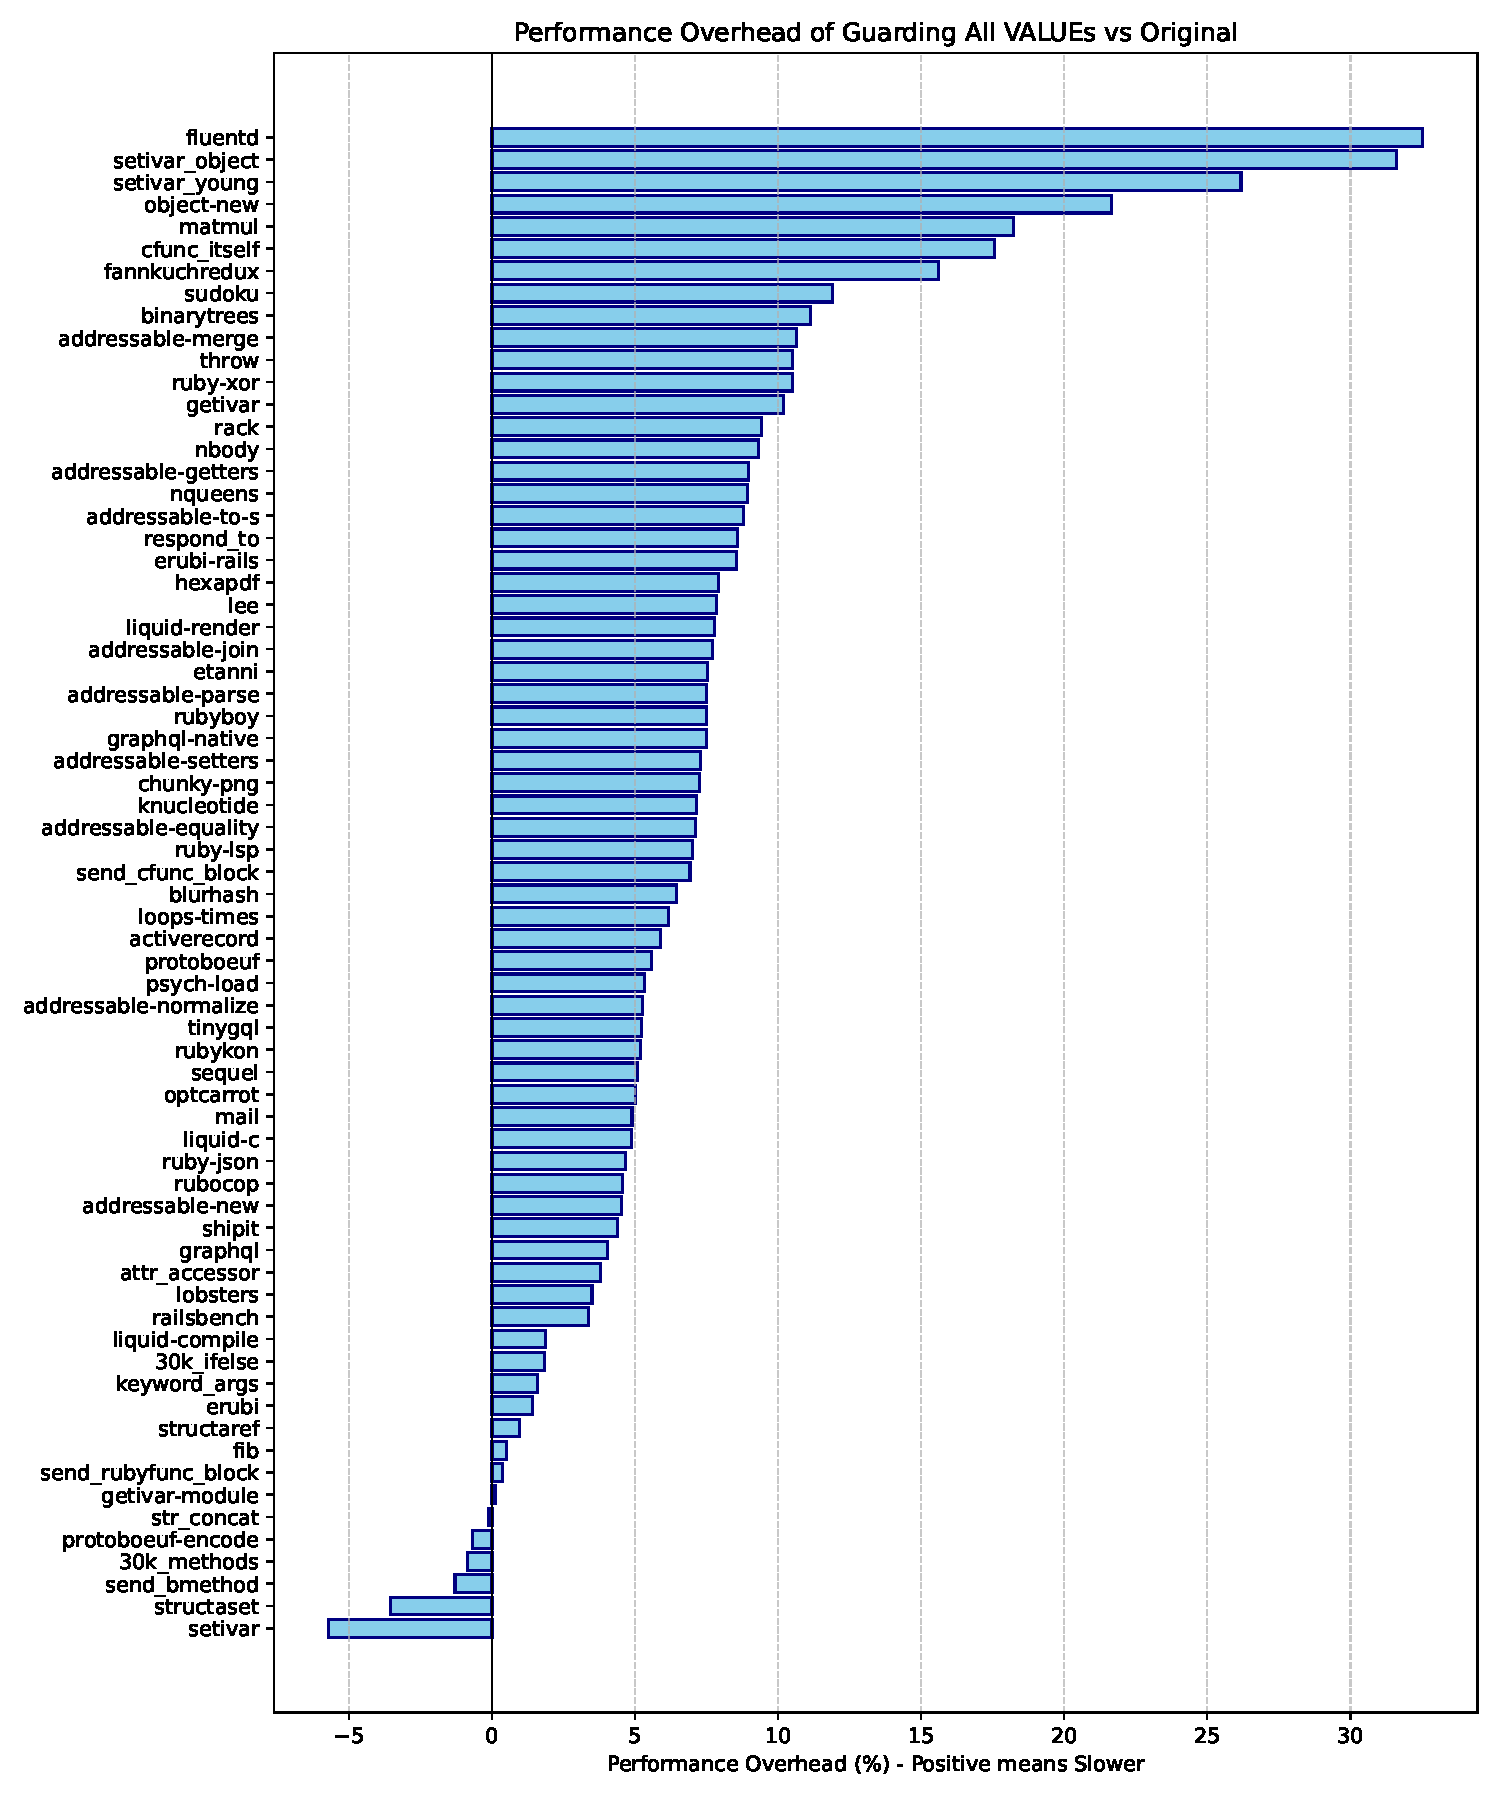
\includegraphics[width=\linewidth]{benchmark_comparison.pdf}
\caption{Performance change from guarding all VALUEs relative to the original CRuby (positive values indicate slowdown).}
\label{fig:benchmark_comparison}
\end{figure}

These results suggest that indiscriminate guarding can harm the interpreter's performance. This motivates a tool that helps focus review on likely omission sites and highlights candidates for cleanup.

In our preliminary runs, all measurements in this section were obtained on a desktop equipped with an AMD Ryzen 7 5700X3D CPU. On this machine, the full GuardLint query set over the CRuby v3.4.5 CodeQL database completed in approximately 1000~s. This order-of-magnitude runtime makes the analysis suitable for practical use, including iterative local runs and potential CI integration.

\section{Discussion}\label{sec:Discussion}

\subsection{Case Study: \texttt{ossl\_cipher\_update}}
We manually inspected representative ``Missing'' reports. One notable case appears in \texttt{ossl\_cipher\_update} in the OpenSSL extension. The  \texttt{data} is initilized through \texttt{rb\_scan\_args}, which is considered to be safe, since the pointer would be held \*\*\*. But, after further inspection, we found that the pattern involves converting an argument with \texttt{StringValue(data)}, creating a new string object and returns a new pointer. Then executing operations that may trigger GC before the subordinate pointer is fully consumed.

We did not reproduce a crash in a with the original CRuby. And we found that the compiler didn't produce binary code that would overwrite the \texttt{data} \texttt{VALUE} in a way that makes it invisible to conservative scanning.

To probe this brittleness, we performed a simulated experiment by explicitly assigning \texttt{Qnil} to \texttt{data} immediately after its last \texttt{VALUE}-level use, approximating an aggressive optimization that removes the root. Under this modification we observed data corruption, indicating that the code can rely on implicit compiler behavior for safety. This result does not by itself demonstrate an exploitable bug in shipping builds, but it motivates closer review and more robust anchoring where appropriate.

Also, we confirmed that even with the simulation, if *** string conversion would not happen, such data corruption would not be observed. Which confirms that speculation of how the pointer is held elsewhere.

\subsection{Limitations}
GuardLint's results are candidates for review rather than definitive proofs of unsafety. Several limitations affect the precision of the analysis.

First, the current implementation is primarily intraprocedural with respect to derived-pointer usage. GuardLint treats passing a subordinate pointer as an argument as a dangerous use, but it does not fully analyze if the actual accesses inside callees are after a GC trigger.

Second, the current implementation doesn't model the actual pointer derivation operation, but *** the approximation that ***.  how the pointer derivations are tracked ***.

Third, some special patterns that needs specific domain knowledge of CRuby's implementation are not *** . For example, how \texttt{VALUE} initialized by \texttt{rb\_scan\_args} is always safe are not ***

Finally, whether the forementioned optimization would happen depends on the build configuration and stack usage ***. Our simulated experiment in the OpenSSL case illustrates that patterns which are safe under one configuration can become problematic under a more aggressive one. The analysis therefore surfaces candidates that merit review rather than providing proofs of either safety or unsafety.

\subsection{Future Work}
Improving precision likely requires better aliasing and path sensitivity, more robust modeling of safe APIs, and explicit handling of common ``implicit anchoring'' idioms. A validated interprocedural analysis of derived-pointer use inside callees would expand coverage for helper-function patterns and callbacks. Finally, packaging GuardLint for CI (with incremental analysis) would enable continuous feedback to developers.

\section{Related Work}\label{sec:Related}
Static analysis for memory safety has evolved significantly, with recent work addressing increasingly complex scenarios. Multiple approaches have been developed for detecting use-after-free bugs: Teodorescu and Lucanu~\cite{static_analysis_use_after_free_cpp} developed frameworks for detecting use-after-free bugs in C++, Yan et al.~\cite{spatio_temporal_context_reduction} introduced spatio-temporal context reduction techniques for scalable UAF detection in multi-MLOC C code, and Caballero et al.~\cite{static_analysis_dangling_pointer} proposed early detection of dangling pointers. Recent comparative studies~\cite{hassler2025comparativestudyfuzzersstatic} evaluate both static analyzers and fuzzers for finding memory unsafety, showing complementarity across tools. These approaches largely focus on explicit memory management rather than conservative-GC settings where subordinate pointers can outlive visible roots.

Closest to our work is Ugawa and Fujimoto's study on detecting mistakes in registering local variables for precise garbage collection in an embedded JavaScript VM (eJSVM) using Coccinelle's control-flow--based pattern matching~\cite{UgawaFujimoto2019PRO}. While the setting is similar, in the case of \texttt{RB\_GC\_GUARD} we must track both derived-pointer extraction and derived-pointer usage, and we must reason about the absence of \texttt{VALUE}-level accesses after potential trigger points.

Empirical evaluations have shown CodeQL's potential for security bug detection, with studies revealing it can detect bug categories missed by other tools~\cite{charoenwet2024empirical}. CodeQL builds upon the foundational QL language~\cite{ql_ecoop} to provide high-level analysis capabilities, and has been used as the basis for domain-specific analyzers such as a resource leak checker for C\# code~\cite{resourceleak_csharp_codeql}. Youn et al.~\cite{codeql_multilingual} extended CodeQL for multilingual program analysis, tracking dataflows across language boundaries.

Recent work has also explored integrating large language models with static analysis. Li et al.\ propose LLift, a framework that uses LLMs to guide static analysis for use-before-initialization bugs in the Linux kernel~\cite{static_analysis_llm}. Paralegal~\cite{paralegal_static_analysis_privacy_bugs} demonstrates that carefully engineered static analyses can be made practical for privacy-bug detection at scale. These lines of work are complementary to GuardLint: they suggest that query-based analyses expressed in CodeQL or similar languages can serve as a foundation for richer, possibly LLM-augmented reasoning about subtle safety properties.

\section{Conclusion}\label{sec:Conclusion}
We presented GuardLint, a CodeQL-based analysis that flags likely missing \texttt{RB\_GC\_GUARD} directives in CRuby's C code. GuardLint identifies patterns where subordinate pointers into object-owned memory may outlive the visibility of their owning \texttt{VALUE} across GC-triggering calls, which can lead to use-after-free under certain compiler optimizations.

On CRuby 3.4.5, GuardLint reported 232 candidate omissions, 265 potentially redundant guards, and 36 existing guards that appear necessary under our model. While some reports depend on build configuration and conservative modeling choices, the results demonstrate that query-based static analysis can systematically surface locations that merit review.

Future work will focus on improving precision through stronger modeling of safe APIs and anchoring idioms, more robust guard detection across compiler implementations, and deeper interprocedural analysis. Ultimately, integrating GuardLint into CI workflows could help prevent regressions and improve the robustness of the CRuby ecosystem against this class of memory safety bugs.

\bibliographystyle{ipsjunsrt}
\bibliography{citations}

\begin{biography}
% Biography placeholders
\end{biography}
\end{document}
